\providecommand{\main}{..}
\documentclass[../COS3712_Notes.tex]{subfiles}

\begin{document}
  \setcounter{chapter}{3}
  \addtocontents{toc}{\protect\newpage}
  \chapter{Viewing}
    \section{Classical and Computer Viewing}
      Projectors meet at the \concept{centre~of~projection~(COP)}.
      The COP corresponds to the centre of the lens in the camera or in the eye,
      and in a computer graphics system, it is the origin of the \concept{camera~frame}
      for perspective views.
      The projection surface is a plane, and the projectors are straight lines.

      Both classical and computer viewing allow the viewer to be an infinite distance
      from the objects.
      As we move the COP to infinity, the projectors become parallel, and the COP can be
      replaced by a \concept{direction~of~projection~(DOP)}.
      Also, as the COP moves to infinity, we can leave the projection plane fixed
      and the size of the image remains about the same, even though the COP is infinitely
      far from the objects.
      Views with a finite COP are called \concept{perspective~views};
      views with a COP at infinity are called \concept{parallel~views}.
      For parallel views, the origin of the camera frame usually lies in the projection plane.

      The class of projections produced by parallel and perspective viewing is known as
      \concept{planar~geometric~projections}, because the projection surface is a plane,
      and the projections are lines.
      Both perspective and parallel projections preserve lines;
      they do not, in general, preserve angles.

    \section{Classical Viewing}
      In classical viewing, there is the underlying notion of a \concept{principal~face}.

      \subsection{Parallel Projections}
        \begin{definition}{Orthographic Projections}
          In all orthographic (or orthogonal) views, the projectors are perpendicular
          to the projection plane.
          In a \concept{multiview orthographic projection}, we make multiple projections,
          in each case with the projection plane parallel to one of the principal faces
          of the object.

          The importance of this type of view is that it preserves both distances and angles
          in faces parallel to the view plane,
          and because there is no distortion of either distance or shape in images of these faces,
          multiview orthographic projections are well suited for working drawings.
        \end{definition}

        \begin{definition}{Axonometric Projections}
          If we want to see more faces of our box-like object in a single view,
          we must remove one of our restrictions.

          In \concept{axonometric views}, the projectors are still orthogonal to the
          projection plane, but the projection plane can have any orientation with respect
          to the object.

          If the projection plane is placed symmetrically with respect to the three
          principal faces, we have an \concept{isometric} view.
          If it is placed symmetrically with respect to two, it is a \concept{dimetric} view.
          The general case is a \concept{trimetric} view.

          In an isometric view, a line segment's length in the image space is shorter
          than its length measured in the object space.
          This \concept{foreshortening} of distances is the same in the three principal directions,
          so we can still make distance measurements.
          In the dimetric view, however, there are two different foreshortening ratios;
          in the trimetric view, there are three.
        \end{definition}

        \begin{definition}{Oblique Projections}
          The \concept{oblique} views are the most general parallel views.
          We obtain an oblique projection by allowing the projectors to make
          an arbitrary angle with the projection plane.
          Consequently, angles in planes parallel to the projection plane are preserved.
          These views are the most difficult to construct by hand.
        \end{definition}

      \subsection{Perspective Projections}
        All perspective views are characterised by \concept{diminution} of size.
        When objects are moved farther from the viewer, their images become smaller.
        This size change gives perspective views their natural appearance;
        however, because the amount by which a line is foreshortened depends on how far
        the line is from the viewer, we cannot make measurements from a perspective view.

        The classical perspective views are known as \concept{one-}, \concept{two-} or
        \concept{three-point perspectives}.
        The differences among the cases are based on how many of the three principal directions
        are parallel to the projection plane.
        The one-, two-, and three- prefixed refer to the number of \concept{vanishing~points}:
        points at which lines of perspective meet.

    \section{Viewing with a Computer}
      In computer graphics, we stress the independence of the object specifications
      and camera parameters.
      Hence, to create one of the classical views, the application program must use information
      about the objects to create and place the proper camera.
      The desired view can be achieved by applying a sequence of transformations on each object
      in the scene.
      Every transformation is equivalent to a change of frames.
      The coordinate types used in the viewing process are object, camera, and clip coordinates.

      Hidden-surface~removal occurs after the fragment shader.
      Although an object might be blocked from the camera by other objects,
      even with hidden-surface~removal enabled, the rasterizer will still generate fragments
      for blocked objects within the clipping volume.

      \begin{sidenote}{Viewing Process Operations}
        There are two operations in the viewing process:
        \begin{enumerate}
          \item Position and orient the camera.
            This operation is the job of the model-view transformation.
            After vertices pass through this transformation, they will be represented
            in eye or camera coordinates.
          \item Applying the projection transformation.
            This step applies the specified projection -- orthographic or perspective --
            to the vertices and puts objects within the specified clipping volume
            into the same clipping cube in clip coordinates.

            One of the functions of either projection will be to allow us to specify a view volume
            in camera coordinates, rather than having to scale our object to fit into the
            default view volume.
        \end{enumerate}
      \end{sidenote}

      The current transformation matrix will be the product of two matrices:
      the \concept{model-view~matrix} and the \concept{projection~matrix}.
      The model-view~matrix will take vertices in object coordinates and convert theme
      to a representation in camera coordinates and thus must encapsulate the positioning
      and orientation of the camera.
      The projection matrix will both carry out the desired projection,
      and convert a viewing volume specified in camera coordinates to fit inside the viewing
      cube in clip coordinates.

      \begin{figure}
        \begin{center}
          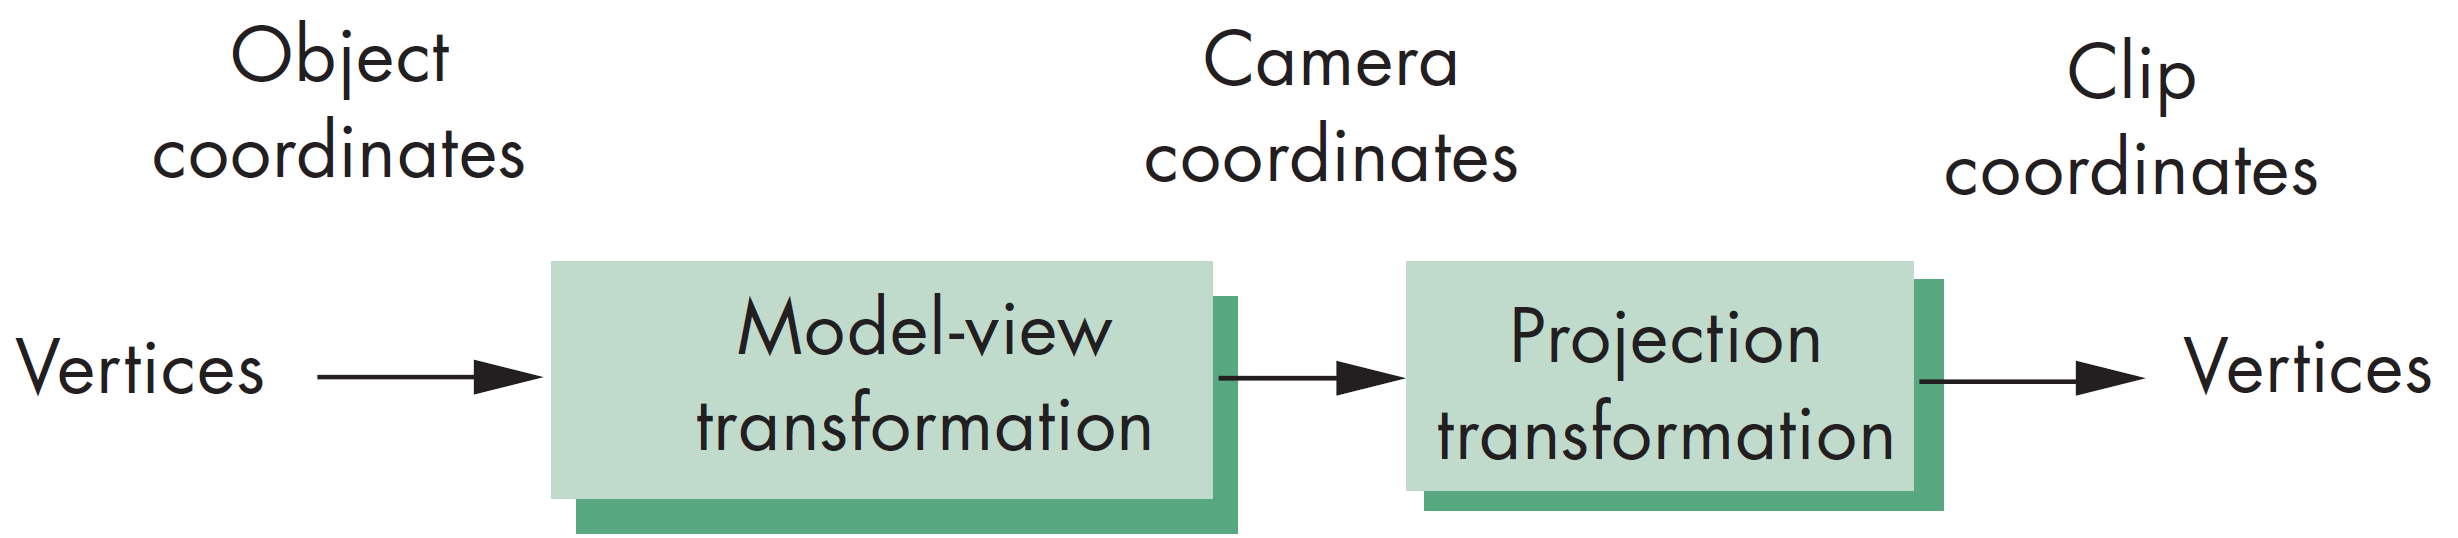
\includegraphics[width=0.8\textwidth]{\main/images/chapter05/viewing_transformations.png}
        \end{center}
        \caption{Viewing Transformations}
      \end{figure}

    \section{Positioning of the Camera}
      \subsection{Positioning of the Camera Frame}
        We can specify vertices in any units we choose, and we can define a model-view~matrix
        as a sequence of affine transformations that repositions these vertices.

        At any given time, the model-view~matrix encapsulates the relationship between the
        camera frame and the object frame.

        The model-view~transformation is the concatenation of two transformations:
        \begin{itemize}
          \item A \concept{modelling transformation} that takes instances of objects
            in model coordinates and brings them into the object frame.
            For each object in a scene, we construct a transformation matrix,
            called the \concept{instance~transformation}, that will scale, orient, and translate
            the object to the desired location in the scene.
            This matrix can be derived by concatenating a series of basic transformation matrices.
          \item A \concept{viewing transformation} that transforms object coordinates
            to eye coordinates.
        \end{itemize}

      \subsection{Constructing the Viewing Transformation}
        There are multiple techniques for specifying the desired position of the camera,
        and implementing camera positioning in WebGL.

        \subsubsection{First Approach: Affine Transformations}
          The first approach is to specify the position indirectly by applying a sequence
          of rotations and translations to the model-view~matrix.
          This approach is a direct application of instance transformation.
          We can think of the camera as being fixed at the origin,
          pointing down the negative $z$-axis.
          Thus, we transform the scene relative to the camera frame.
          We usually want to specify the camera's position \emph{before} we position any objects
          in the scene.
          The order of transformations on the camera may appear to be backward from what you might
          expect.

        \subsubsection{Second Approach: View-Orientation Matrix}
          A second approach is to describe the camera's position and orientation
          in the world frame.
          We construct the matrix, called the \concept{view-orientation~matrix},
          that will take us from world coordinates to camera coordinates.
          The precise type of image we wish to obtain is determined separately by the
          specification of the projection matrix.
          This second part of the viewing process is often called the
          \concept{normalisation~transformation}.

          We approach this problem as one of a change in frames.
          We think of the camera as positioned initially at the origin, pointing in the
          negative $z$ direction.

          \begin{sidenote}{Parameters Needed for Specifying the Camera Frame}
            $ $\vspace{-1em}
            \begin{descriptimize}
              \item[View Reference Point (VRP)] The desired location of the camera, or COP,
                whose position is given in the world frame
                (i.e. specified in world coordinates).
              \item[View-Plane Normal (VPN)] Gives the orientation of the projection plane
                or back of the camera.
                Specifies the normal of the projection plane, known as $\mathbf{n}$.
              \item[View-Up Vector (VUP)] Specifies the direction that is `up' from the
                camera's perspective.
                This vector is \emph{not necessarily} orthogonal to $\mathbf{n}$.
            \end{descriptimize}
          \end{sidenote}

          We project the VUP vector onto the view plane to obtain the up-direction vector
          $\mathbf{v}$, which is orthogonal to $\mathbf{n}$.
          We then use the cross product $\mathbf{v} \times \mathbf{n}$ to obtain
          a third orthogonal direction $\mathbf{u}$.
          This new orthogonal coordinate system is referred to as the
          \concept{viewing-coordinate system} or the \concept{$\mathbf{u}$-$\mathbf{v}$-$\mathbf{n}$ system}.
          With the addition of the VRP, we have the desired camera frame.

        \subsubsection{Third Approach: The Look-At Function}
          Similar to the second approach: it differs only in the way we specify the VPN.
          A camera is located at a point $\mathbf{e}$, called the \concept{eye~point},
          specified in the world frame, equivalent to the VRP above.
          The camera is pointed at a second point $\mathbf{a}$, called the \concept{at~point}.
          The VPN is given by the vector formed by point subtraction between the eye~point
          and the at~point, and normalising it.
          \begin{align*}
            \mathbf{vpn} &= \mathbf{a} - \mathbf{e} &
            \mathbf{n} &= \frac{\mathbf{vpn}}{\lvert \mathbf{vpn} \rvert}
          \end{align*}

    \section{Parallel Projections}
      \concept{Projection} is a technique that takes the specification of points in
      three dimensions and maps them to points on a two-dimensional projection surface.
      Such a transformation is not invertible, because all points along a projector
      map into the same points on the projection surface.

      A \concept{parallel~projection} is the limit of a perspective projection in which the
      centre of projection is infinitely far from the objects being viewed,
      resulting in projectors that are parallel rather than converging at the centre of projection.

      \subsection{Orthogonal Projections}
        \concept{Orthogonal} or \concept{orthographic} projections are a special case
        of parallel projections in which the projectors are perpendicular to the view plane.
        In terms of a camera, orthogonal projections correspond to a camera with a back plane
        parallel to the lens, which has an infinite focal length.

      \subsection{Projection Normalisation}
        \concept{Projection~normalisation} is a technique that converts all projections
        into orthogonal projections by first distorting the objects such that the
        orthogonal projection of the distorted objects is the same as the desired projection
        of the original objects.

        \begin{definition}{Canonical View Volume}
          The cube defined by the planes
          \begin{align*}
            x &= \pm 1 & y &= \pm 1 & z &= \pm 1
          \end{align*}
        \end{definition}

        The \concept{normalisation~matrix} should be defined such that it transforms (distorts)
        the specified view volume to coincide directly with the \concept{canonical} (default)
        view volume.
        So, vertices are transformed such that vertices within the specified view volume
        are transformed into vertices within the canonical view volume,
        and vertices outside the specified view volume are transformed to vertices outside
        the canonical view volume.

        The concatenation of the normalisation~matrix, which carries out the distortion,
        and the simple orthogonal projection matrix, yields a homogeneous coordinate matrix
        that produces the desired projection.

        \begin{sidenote}{Advantages of Projection Normalisation}
          $ $\vspace{-1em}
          \begin{itemize}
            \item Both perspective and parallel views are supported by the same pipeline
              by loading in the proper normalisation matrix.
            \item The canonical view volume simplifies the clipping process,
              because the sides are aligned with the coordinate axes.
          \end{itemize}
        \end{sidenote}

        The normalisation process defines what most systems call the \concept{projection~matrix}.
        The projection matrix brings objects into four-dimensional clip coordinates,
        and the subsequent perspective division converts vertices to a representation
        in three-dimensional normalised device coordinates.
        Values in normalised device coordinates are later mapped to window coordinates
        by the viewport transformation.

      \subsection{Orthogonal Projection Matrices}
        The shape of the viewing volume for an orthogonal projection is a right-parallelepiped.

        \begin{sidenote}{Projection Normalisation Process for an Orthographic Projection}
          $ $\vspace{-1em}
          \begin{enumerate}
            \item Move the centre of the specified view volume to the centre of the canonical
              view volume (the origin) by doing a translation.
            \item Scale the sides of the specified view volume to each have a length of 2.
          \end{enumerate}
        \end{sidenote}

    \section{Perspective Projections}
      A point in space $(x, y, z)$ is projected along a projector into the point
      $(x_p, y_p, z_p)$.
      All projectors pass through the origin, and, because the projection is perpendicular
      to the $z$-axis:
      \begin{align*}
        z_p = d
      \end{align*}
      Because the camera is pointing in the negative $z$ direction,
      the projection plane is in the negative half-space $z < 0$,
      and the value of $d$ is negative.

      \begin{figure}[b]
        \begin{center}
          \begin{subfigure}{0.3\textwidth}
            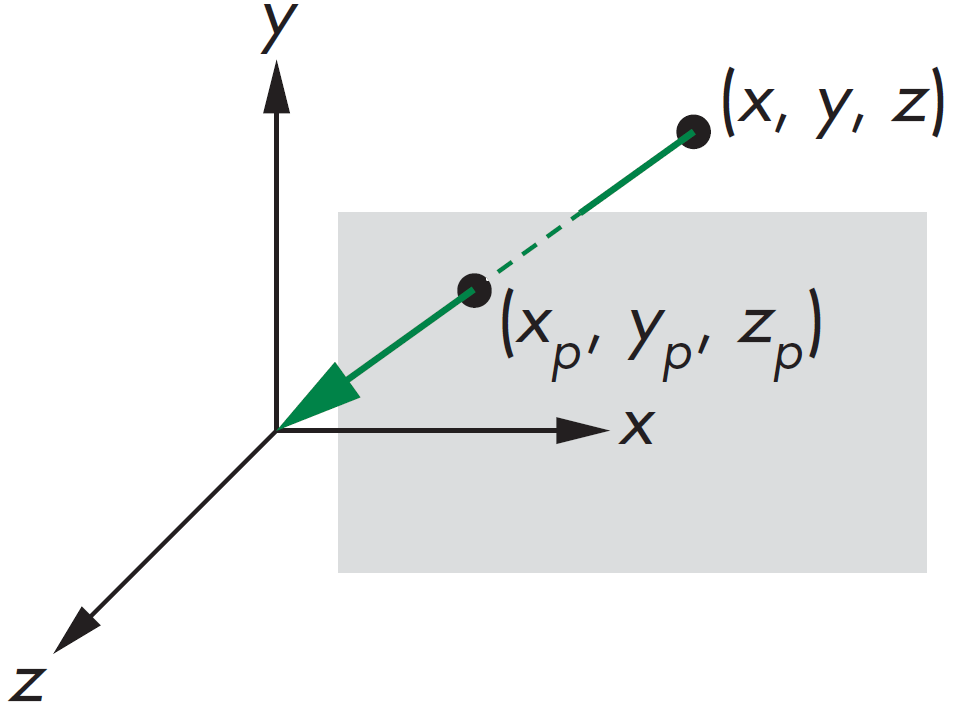
\includegraphics[width=\textwidth]{images/chapter05/perspective_3d.png}
            \caption{3D View}
          \end{subfigure}
          \begin{subfigure}{0.3\textwidth}
            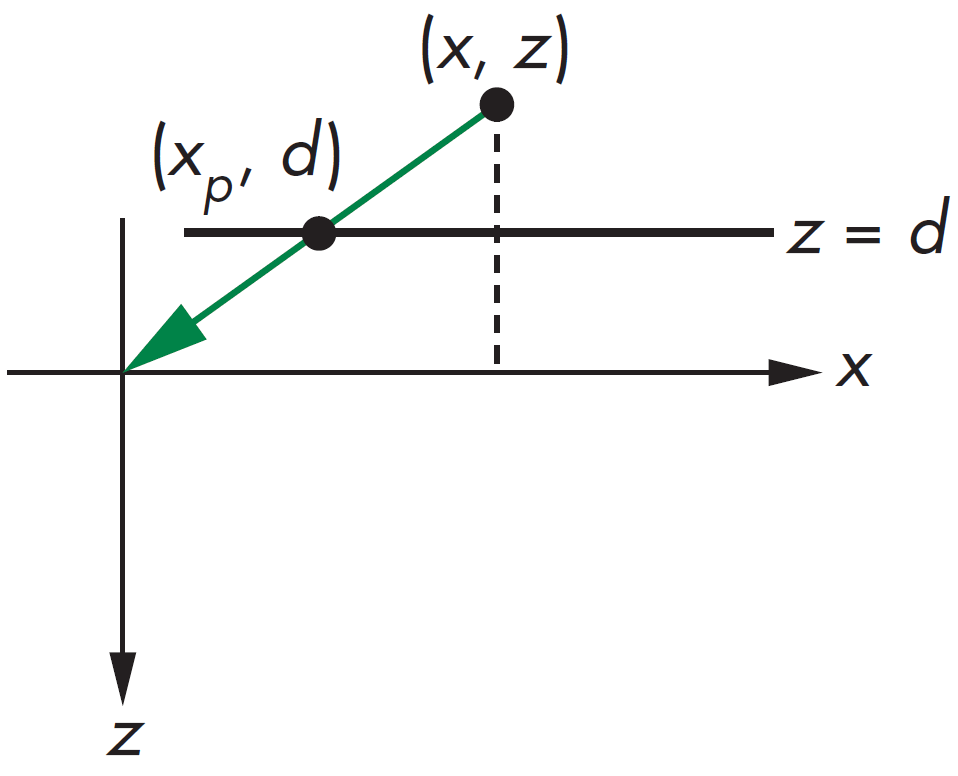
\includegraphics[width=\textwidth]{images/chapter05/perspective_top.png}
            \caption{Top View}
            \label{persp:b}
          \end{subfigure}
          \begin{subfigure}{0.3\textwidth}
            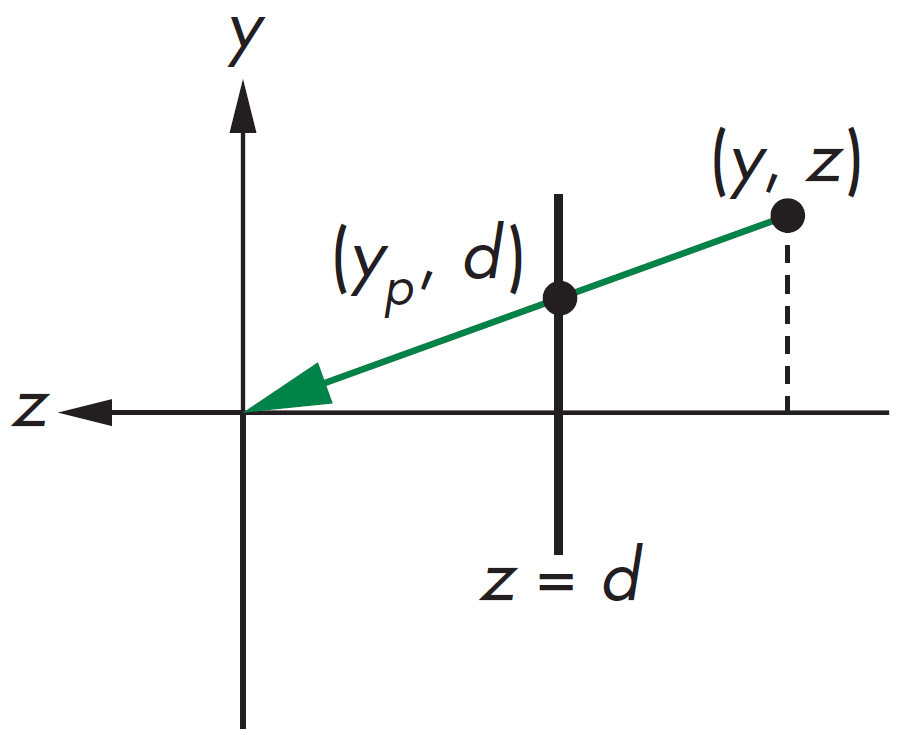
\includegraphics[width=\textwidth]{images/chapter05/perspective_side.png}
            \caption{Side View}
            \label{persp:c}
          \end{subfigure}
        \end{center}
        \caption{Three views of perspective projection.}
      \end{figure}

      From the top view in \autoref{persp:b}, we see two similar triangles
      whose tangents must be the same.
      \begin{align*}
        \frac{x_p}{d} &= \frac{x}{z}\\
        \Rightarrow x_p &= \frac{x}{z/d}
      \end{align*}
      (This seems unintuitive, but multiplying by $d$ is the same as dividing by $1/d$.)

      Using the side view in \autoref{persp:c}:
      \begin{align*}
        \frac{y_p}{d} &= \frac{y}{z}\\
        \Rightarrow y_p &= \frac{y}{z/d}
      \end{align*}

      These equations are non-linear.
      The division by $z$ describes \concept{nonuniform~foreshortening}:
      the images of objects farther from the centre of projection are reduced in size
      (\concept{diminution}) compared to the images of objects closer to the COP.

      Although this \concept{perspective~transformation} preserves lines,
      it is not affine.
      It is also irreversible.
      Because all points along a projector project into the same point,
      we cannot recover a point from its projection.

      We can extend our use of homogeneous coordinates to handle projections.
      Originally, we represented a point with $(x, y, z)$ with $(x, y, z, 1)$.
      Instead, we can replace $(x, y, z)$ with the four-dimensional point
      \begin{align*}
        \mathbf{p} = \begin{bmatrix}
          wx \\
          wy \\
          wz \\
          w
        \end{bmatrix}.
      \end{align*}
      As long as $w \neq 0$, we can recover the three-dimensional point from its four-dimensional
      representation by dividing the first three components by $w$.
      In this new form, points in three dimensions become lines through the origin
      in four dimensions.
      Transformations are again represented by $4 \times 4$ matrices,
      but now the final row of the matrix can be altered
      -- and thus $w$ can be changed by such a transformation.

      Consider the matrix
      \begin{align*}
        \mathbf{M} = \begin{bmatrix}
          1 & 0 & 0 & 0 \\
          0 & 1 & 0 & 0 \\
          0 & 0 & 1 & 0 \\
          0 & 0 & 1/d & 0
        \end{bmatrix}.
      \end{align*}
      This matrix transforms the point
      \begin{align*}
        \mathbf{p} = \begin{bmatrix}
          x \\
          y \\
          z \\
          1
        \end{bmatrix}
      \end{align*}
      to the point
      \begin{align*}
        \mathbf{q} = \begin{bmatrix}
          x \\
          y \\
          z \\
          z/d
        \end{bmatrix}.
      \end{align*}

      By performing \concept{perspective~division}
      (dividing the first three components by the fourth),
      we obtain
      \begin{align*}
        \begin{bmatrix}
          \frac{x}{z/d} \\
          \frac{y}{z/d} \\
          \frac{z}{z/d} \\
          1
        \end{bmatrix} &=
        \begin{bmatrix}
          x_p \\
          y_p \\
          z_p \\
          1
        \end{bmatrix}
      \end{align*}
      So, matrix $\mathbf{M}$ can be used to perform a simple perspective projection.

      We apply the projection matrix after the model-view matrix, but must perform
      perspective division at the end.

    \section{Perspective Projections with WebGL}
      The projections developed earlier did not take into account the properties of the camera:
      the focal length of its lens or the size of the film plane.
      We did not include the effects of clipping.

      With most graphics APIs, the application program specifies clipping parameters through the
      specification of a projection.
      The infinite pyramid becomes a finite clipping volume by adding front and back clipping
      planes, as well as the angle of view.
      The resulting view volume is a \concept{frustum}: a truncated pyramid.

      Two APIs for specifying a perspective projection matrix are \mintinline{javascript}{frustum()}
      and \mintinline{javascript}{perspective()}.

    \section{Perspective Projection Matrices}
      For perspective matrices, we follow a path similar to the one used for parallel projections:
      find a transformation that allows us, by distorting the vertices of our objects,
      to do a simple canonical projection to obtain the desired image.
      Our first step is to decide what this canonical viewing volume should be.
      We then introduce a new transformation, the \concept{perspective~normalisation~transformation}
      that converts a perspective projection to an orthogonal projection.

    \section{Hidden Surface Removal}
      The graphics system must be careful about which surfaces it displays.
      Conceptually, we seek algorithms that either remove those surfaces that should not be
      visible to the viewer (\concept{hidden-surface removal algorithms}),
      or find which surfaces are visible (\concept{visible-surface algorithms}).

      \begin{sidenote}{Types of Hidden Surface Removal Algorithms}
        $ $\vspace{-1em}
        \begin{descriptimize}
          \item[Object-Space Algorithms] Attempt to order the surfaces of the objects
            in the scene such that rendering surfaces in a particular order provides
            the correct image.

            This class of algorithms does not work well with pipelines architectures
            in which objects are passed down the pipeline in an arbitrary order.
            In order to decide on a proper order in which to render the objects,
            the graphics system must have all the objects available,
            so it can sort them into the desired back to front order.
          \item[Image-Space Algorithms] Work as part of the projection process
            and seek to determine the relationship among object points on each projector.
            The $z$-buffer algorithm is of this type,
            and fits well with the rendering pipeline in most graphics systems,
            because we can save partial information as each object is rendered.
        \end{descriptimize}
      \end{sidenote}

      \begin{definition}{$Z$-Buffer Algorithm}
        As primitives are rasterized, we keep track of the distance from the COP
        or the projection plane to the closest point on each projector that has already
        been rendered.
        We update this information as successive primitives are projected and filled.
        Ultimately, we display only the closest point on each projector.
        The algorithm requires a \concept{depth buffer} (or \concept{$z$-buffer})
        to store the necessary depth information as primitives are rasterized.
        The $z$-buffer forms part of the framebuffer, and has the same spatial resolution
        as the colour buffer.
      \end{definition}

      \begin{sidenote}{Advantages of $Z$-Buffer}
        $ $\vspace{-1em}
        \begin{itemize}
          \item Its complexity is proportional to the number of fragments generated
            by the rasterizer.
          \item It can be implemented with a small number of additional calculations
            over what we have to do to project and display polygons without
            hidden-surface removal.
        \end{itemize}
      \end{sidenote}

      \subsection{Culling}
        For a convex object, faces whose normals point away from the viewer are never visible,
        and an be eliminated (or \concept{culled}) before the rasterizer.

        The default is to cull back faces.
        However, back face culling is guaranteed to produce a correct image only if we have
        a single convex object.

    \section{Displaying Meshes}
      A \concept{mesh} is a set of polygons that share vertices and edges.
      A general mesh may contain polygons with any number of vertices,
      and requires a moderately sophisticated data~structure to store and display efficiently.
      Rectangular and triangular meshes are much simpler to work with,
      and are useful for a wide variety of applications.

      Rectangular meshes can be used to display height~data.
      \concept{Height~data} determine a surface, such as terrain,
      either through a function that gives the heights above a reference value,
      such as elevations above sea~level,
      or through samples taken at various points on the surface.

      We should strive to organise this data in a way that will allow us to draw it using
      a combination of triangle~strips and triangle~fans.

    \section{Projections and Shadows}
      Although shadows are not geometric objects, they are important components of realistic
      images, and give many visual clues to the spatial relationships among the objects
      in a scene.

      Starting from a physical point of view, shadows require a \concept{light~source}
      to be present.
      A point is in shadow if it is not illuminated by any light source,
      or, equivalently, if a viewer at that point cannot see any light sources.
      However, if the only light source is at the centre of projection, there are no visible
      shadows, because any shadows are behind visible objects.
      This lighting strategy has been called the \concept{`flashlight~in~the~eye'~model}.

      To add physically correct shadows, we must understand the interaction between
      light and materials.

      \pagebreak

      \subsection{Projected Shadows}
        \begin{figure}
          \begin{center}
            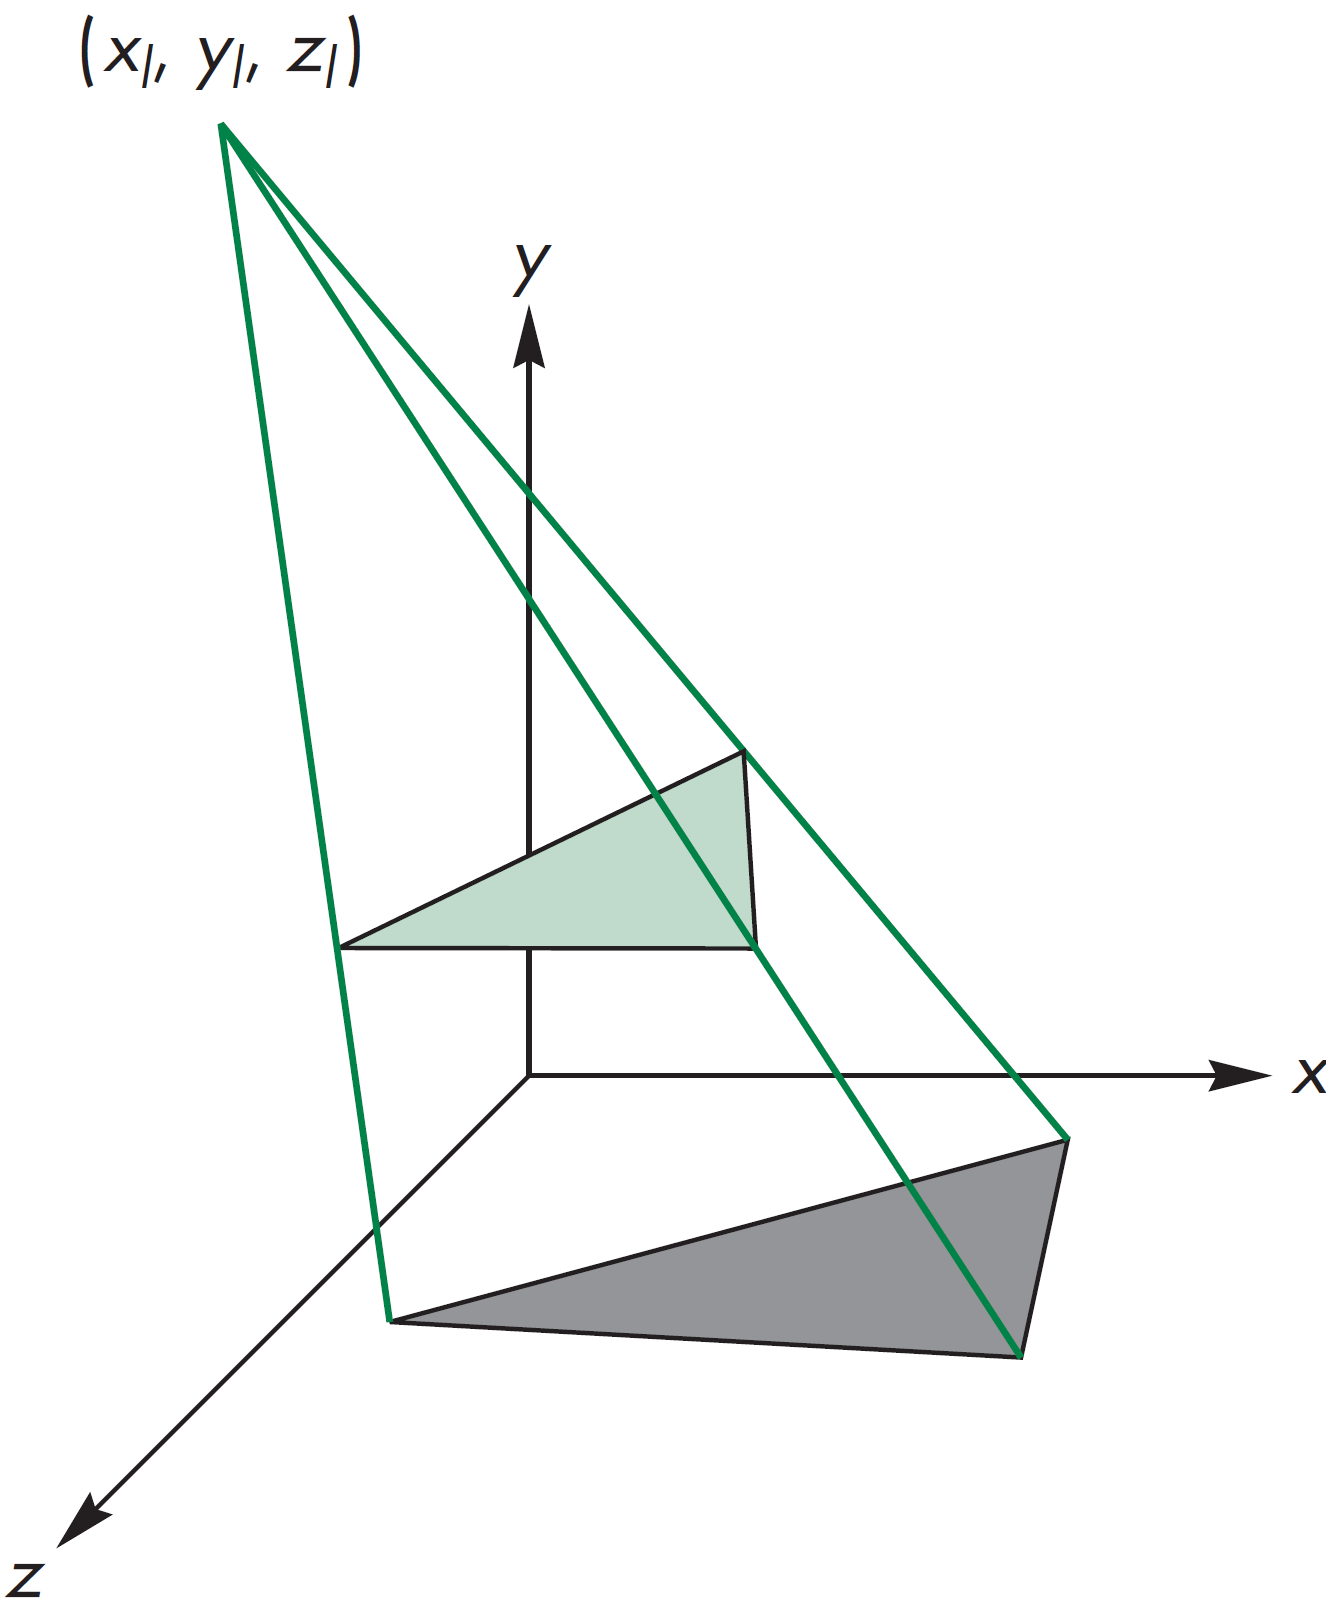
\includegraphics[height=5cm]{\main/images/chapter05/shadow.png}
          \end{center}
          \caption{Shadow from a single polygon.}
          \label{fig:shadow}
        \end{figure}

        Consider the shadow generated by a point source in \autoref{fig:shadow}.
        We assume for simplicity that the shadow falls on a flat ground that can be described
        by the equation
        \begin{align*}
          y = 0.
        \end{align*}
        Not only is the shadow a flat polygon -- called a \concept{shadow polygon} --
        but it is also a projection of the original polygon onto the surface.
        Specifically, the shadow polygon is the projection of the polygon onto the surface
        with the centre of projection at the light source.
        Thus, if we do a projection onto the plane of a surface in a frame in which
        the light source is at the origin, we obtain the vertices of the shadow polygon.
        These vertices must then be converted back to a representation in the world frame.
        We can find a suitable projection matrix and use it to compute the vertices
        of the shadow polygon.

    \rulechapterend

\end{document}
